\chapter*{Ход работы}

\section*{Функциональная схема разрабатываемой системы на кристалле}
На рисунке 1 изображена функциональная схема разрабатываемой системы на кристалле.

\FloatBarrier
\begin{figure}[h]
	\begin{center}
		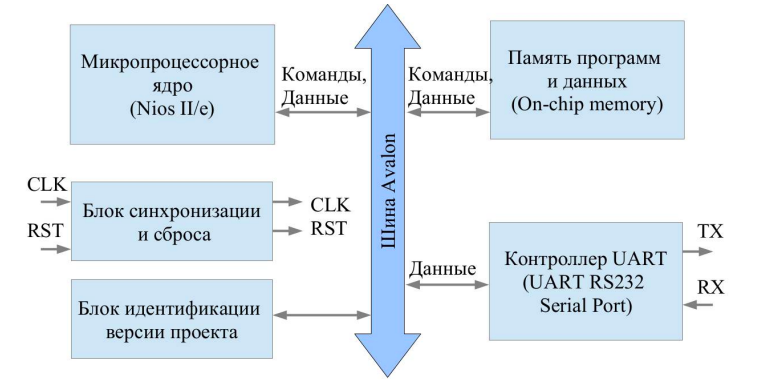
\includegraphics[width=\linewidth]{inc/func.png}
	\end{center}
	\caption{Функциональная схема разрабатываемой системы на кристалле}
\end{figure}
\FloatBarrier

Основные составляющие системы на кристалле:
\begin{enumerate}
	\item Микропроцессорное ядро Nios II/e выполняет функции управления системой.
	\item Внутренняя оперативная память СНК, используемая для хранения программы управления и данных;
	\item Системная шина Avalon обеспечивает связность всех компонентов системы.
	\item Блок синхронизации и сброса обеспечивает обработку входных сигналов сброса и синхронизации и распределение их в системе.
	\item Блок идентификации версии проекта обеспечивает хранение и выдачу уникального
	идентификатора версии, который используется программой управления при
	инициализации системы.
	\item Контроллер UART обеспечивает прием и передачу информации по интерфейсу RS232.
\end{enumerate}

\section*{Создание нового модуля системы на кристалле QSYS}
Были проделаны следующие действия:
\begin{enumerate}
	\item Создан новый модуль QSYS.
	\item Установлена частота внешнего сигнала синхронизации -- $5 * 10^7 Гц$.
	\item Добавлен в проект модуль синхронизируемого микропроцессорного ядра Nios2.
	\item Выбран тип ядра Nios2/e.
	\item Добавлен в проект модуль ОЗУ программ и данных.
	\item Добавлены компоненты Avalon System ID и Avalon UART.
	\item Создана сеть синхронизации и сброса системы.
	\item Все блоки подключены к системной шине.
	\item Экспортированы сигналы TX и RX во внешние порты.
	\item Выполнена настройка таблицы прерываний процессора.
	\item Назначить базовые адреса устройств.
\end{enumerate}

Конечное состояние окна модуля QSYS изображено на рисунке 2:

\FloatBarrier
\begin{figure}[h]
	\begin{center}
		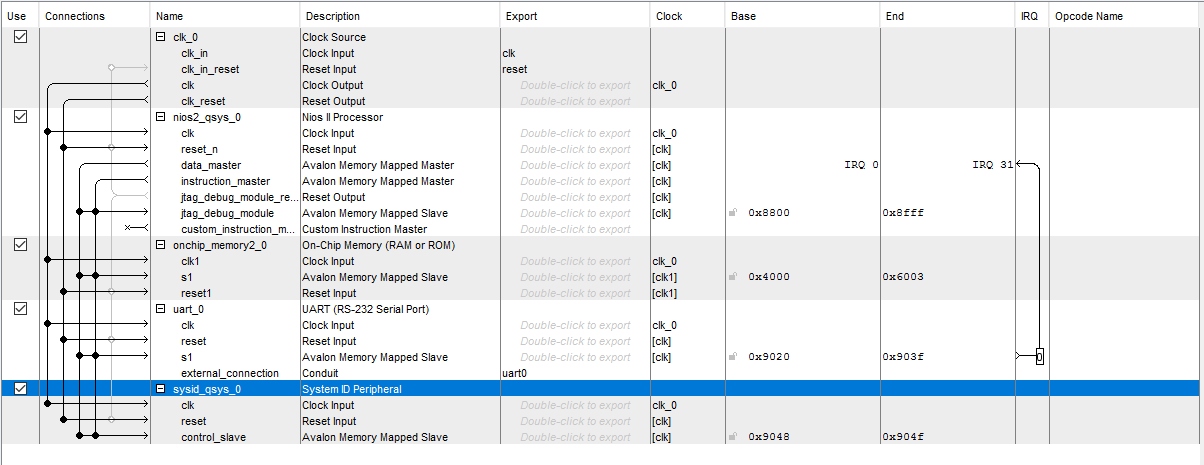
\includegraphics[width=\linewidth]{inc/qsys.png}
	\end{center}
	\caption{Конечное состояние окна модуля QSYS}
\end{figure}
\FloatBarrier

\section*{Модуль Pin Planner}
Портам проекта назначены контакты микросхемы.

На рисунке 3 изображён общий вид модуля Pin Planner. 

\FloatBarrier
\begin{figure}[]
	\begin{center}
		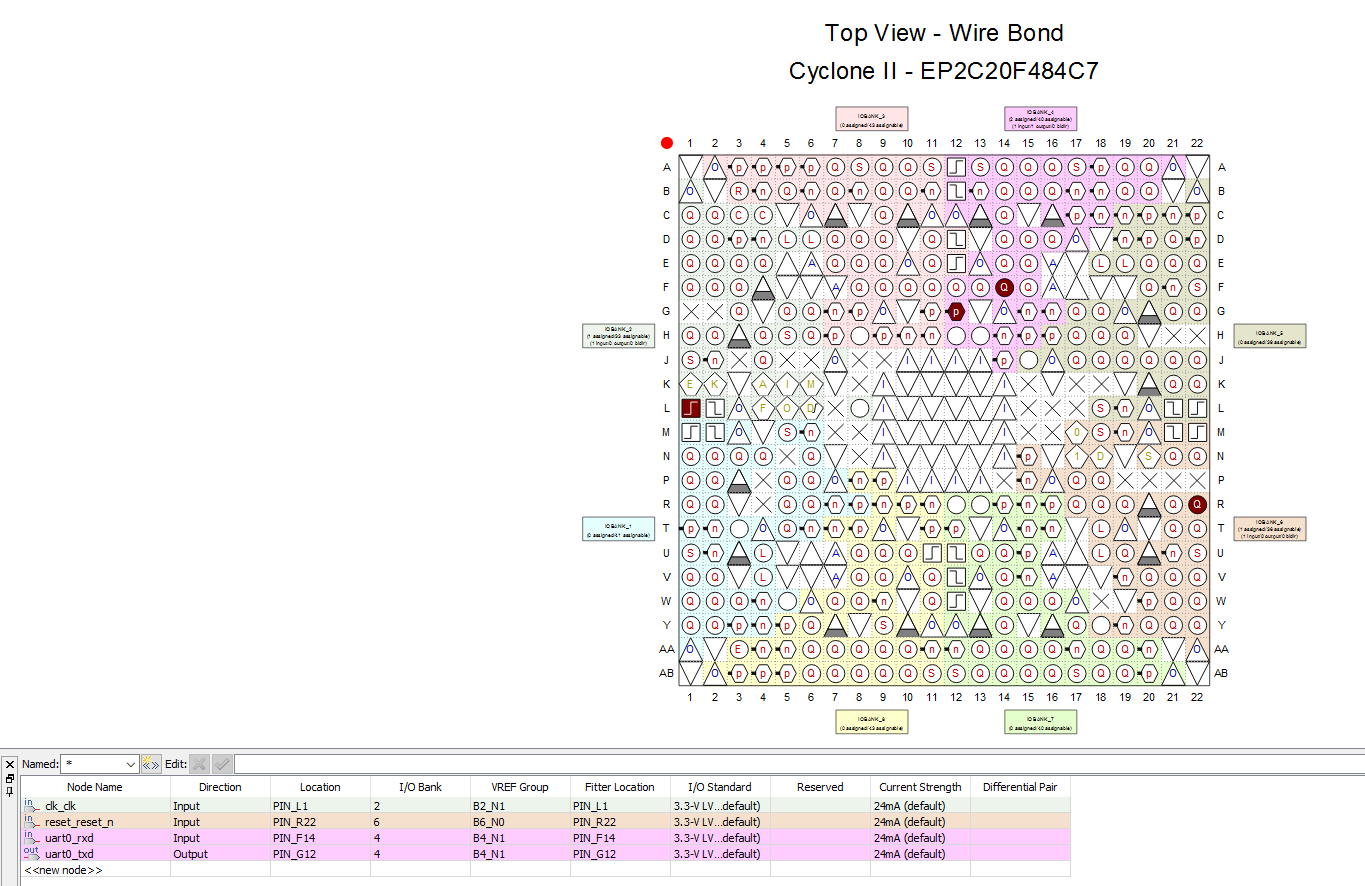
\includegraphics[width=\linewidth, height=7cm]{inc/pinplan.png}
	\end{center}
	\caption{Общий вид модуля Pin Planner}
\end{figure}
\FloatBarrier

На рисунке 4 изображены назначения портам проекта контактов микросхемы.

\FloatBarrier
\begin{figure}[h]
	\begin{center}
		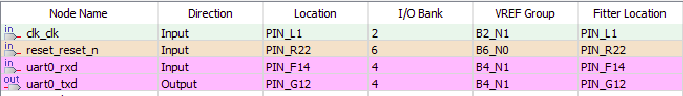
\includegraphics[width=\linewidth]{inc/pins.png}
	\end{center}
	\caption{Назначение портам проекта контактов микросхемы}
\end{figure}
\FloatBarrier

\section*{Таблица распределения адресов}
На рисунке 5 изображена таблица распределения адресов из программы.
\FloatBarrier
\begin{figure}[]
	\begin{center}
		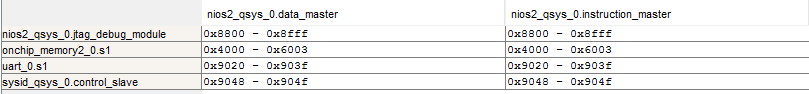
\includegraphics[width=\linewidth]{inc/map.png}
	\end{center}
	\caption{Таблица распределения адресов}
\end{figure}
\FloatBarrier
